
\documentclass[10pt]{standalone}
\input{../tikzpic_packages.tex}
\begin{document}
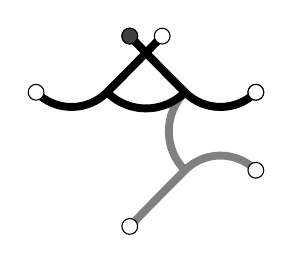
\begin{tikzpicture}
\tikzset{
    part/.style={line width = 1mm, color=\col},
    foot/.style={fill=white},
    footfixed/.style={fill=darkgray},
    grid line/.style={white},
    start line/.style={help lines}}
\def\rfoot{.1}

\def\col{gray}
\def\alpi{1.000000}
\def\beti{90.000000}
\def\gam{90.000000}
\def\alpii{1.000000}
\def\betii{90.000000}
\def\gamh{45.000000}

\def\eps{90.000000}
\def\ci{44.000000}
\def\cii{135.000000}
\def\ciii{316.000000}
\def\civ{225.000000}

\def\ri{57.295780}
\def\rii{0.636620}
\def\rg{0.700282}
\def\riii{57.295780}
\def\riv{0.636620}

\path (0.000000, 0.000000)coordinate(F1);

\draw[part] (F1)arc(180+\ci:180+\ci+\alpi:\ri)coordinate(OM);
\draw[part] (OM)arc(180+\ci+\alpi:180+\ci+\alpi+\beti:\rii)coordinate(F2);
\draw[part] (OM)arc(90+\ci+\alpi:90+\ci+\alpi+\gam:\rg)coordinate(UM);
\draw[part] (UM)arc(\gam+\ci+\alpi:\gam+\ci+\alpi+\alpii:\riii)coordinate(F3);
\draw[part] (UM)arc(\gam+\ci+\alpi:\gam+\ci+\alpi-\betii:\riv)coordinate(F4);

\draw[foot] (0.000000, 0.000000)circle(\rfoot);
\draw[foot] (1.601217, -0.713241)circle(\rfoot);
\draw[foot] (0.000000, -2.416831)circle(\rfoot);
\draw[foot] (1.601217, -1.703589)circle(\rfoot);





\def\col{black}
\def\alpi{1.000000}
\def\beti{90.000000}
\def\gam{-90.000000}
\def\alpii{1.000000}
\def\betii{90.000000}
\def\gamh{-45.000000}

\def\eps{90.000000}
\def\ci{134.000000-90}
\def\cii{225.000000}
\def\ciii{226.000000}
\def\civ{135.000000}

\def\ri{57.295780}
\def\rii{0.636620}
\def\rg{-0.700282}
\def\riii{57.295780}
\def\riv{0.636620}

\path (0.000000, 0)coordinate(F1);

\draw[part] (F1)arc(180+\ci:180+\ci+\alpi:\ri)coordinate(OM);
\draw[part] (OM)arc(180+\ci+\alpi:180+\ci+\alpi+\beti:\rii)coordinate(F2);
\draw[part] (OM)arc(90+\ci+\alpi:90+\ci+\alpi+\gam:\rg)coordinate(UM);
\draw[part] (UM)arc(\gam+\ci+\alpi:\gam+\ci+\alpi+\alpii:\riii)coordinate(F3);
\draw[part] (UM)arc(\gam+\ci+\alpi:\gam+\ci+\alpi-\betii:\riv)coordinate(F4);

\draw[footfixed]  (F1)circle(\rfoot);
\draw[foot]  (F2)circle(\rfoot);
\draw[foot] (F3)circle(\rfoot);
\draw[foot] (F4)circle(\rfoot);

\end{tikzpicture}
\end{document}
